\documentclass{sig-alternate}
\usepackage{color}
\usepackage[colorinlistoftodos]{todonotes}
\usepackage{amssymb}
\usepackage{upgreek}
\begin{document}
\conferenceinfo{UMM CSci Senior Seminar Conference, December 2014}{Morris, MN}

\title{Gait Recognition in Mobile Security}

\numberofauthors{1}

\author{
\alignauthor
Chase R. Ottomoeller\\
	\affaddr{Division of Science and Mathematics}\\
	\affaddr{University of Minnesota, Morris}\\
	\affaddr{Morris, Minnesota, USA 56267}\\
	\email{ottom005@morris.umn.edu}
}

\maketitle



%----------------------------------------------------------------------------------------------------------------------%
\begin{abstract}
This paper discusses a new form of mobile security, emphasizing both security and usability. Having a form of security of a mobile device that is unobtrusive can make that device easier to use. Using built-in accelerometers in smart phones as a way to collect biometric data is one of these forms. In this case the biometric data is a person's gait, or walking pattern. This increases the security of the device by allowing the authentication to not be something you have or something you know, but something you are. There are two example that this paper will compare showing two forms of gait analysis. Though both examples need further work, they both implement working security schemes allowing the phone to  verify the users identity correctly.  
\end{abstract}

\keywords{mobile authentication, gait recognition, biometrics, accelerometer}



%----------------------------------------------------------------------------------------------------------------------%
\section{Introduction}
	Computational power in computers continues to increase year to year. One growing concern is security, including the security of mobile devices such as smart phones. The current methods to unlock smart phones will soon be vulnerable to brute force  attack (trying all possible combinations). Common security authentication methods include: pin, password, swipe lock, token, and fingerprint. Most of these methods are either something a person has (card, token, key) or something a person knows(password). They all require a physical action to unlock the phone. A new form of mobile security involves biometrics. Using biometrics allows to identify a person based on their characteristics (fingerprint) and not by what they have or what they know.  One form of biometrics being explored uses a person's gait (walking patter). 
	%This  making it an unobtrusive form of security.
	
	
	  
	 
	 
	
	This paper analyzes two different approaches for gait extraction and analysis. Each approach uses a general process to extract and analyse the data which includes: Pre-processing, Feature Extraction, and Gait Analysis. \textit{Pre-processing} is the process of taking the raw accelerometer data and preparing it for feature extraction. \textit{Feature Extraction} is taking the pre-processed biometric data, and locating distinctive characteristics within that data. \textit{Gait Analysis} is taking the features extracted from the data, and comparing them against a predefined template. This comparison is what determines if the current user is an imposter or not.

	In the following sections, I will be comparing two approaches of gait recognition using accelerometers from a mobile device, such as a smart phone. These two approaches use different placement of the mobile device on the body. This difference in placement impacts the techniques that are used to recognize and analyze gait patterns. One approach has the smart phone in a fixed location on the waist. I will refer to this method as the \textit{fixed} method. The other method has the smart phone in a more natural position on the body such as in a pocket. This method will be referred to as the \textit{unfixed} method. Though both methods use a complex approach shown in figure~\ref{fig:AlgorithmProcess}, I will simplify comparisons between these methods. I will group them into three categories: Pre-Processing, Feature Extraction, and Gait Analysis. 
	
%\begi%@@@@@@@@@@@@@@@@@@@@@@@@@@@@@@@@@@@@@@@@@@@@@@@@%
\begin{figure}
\centering
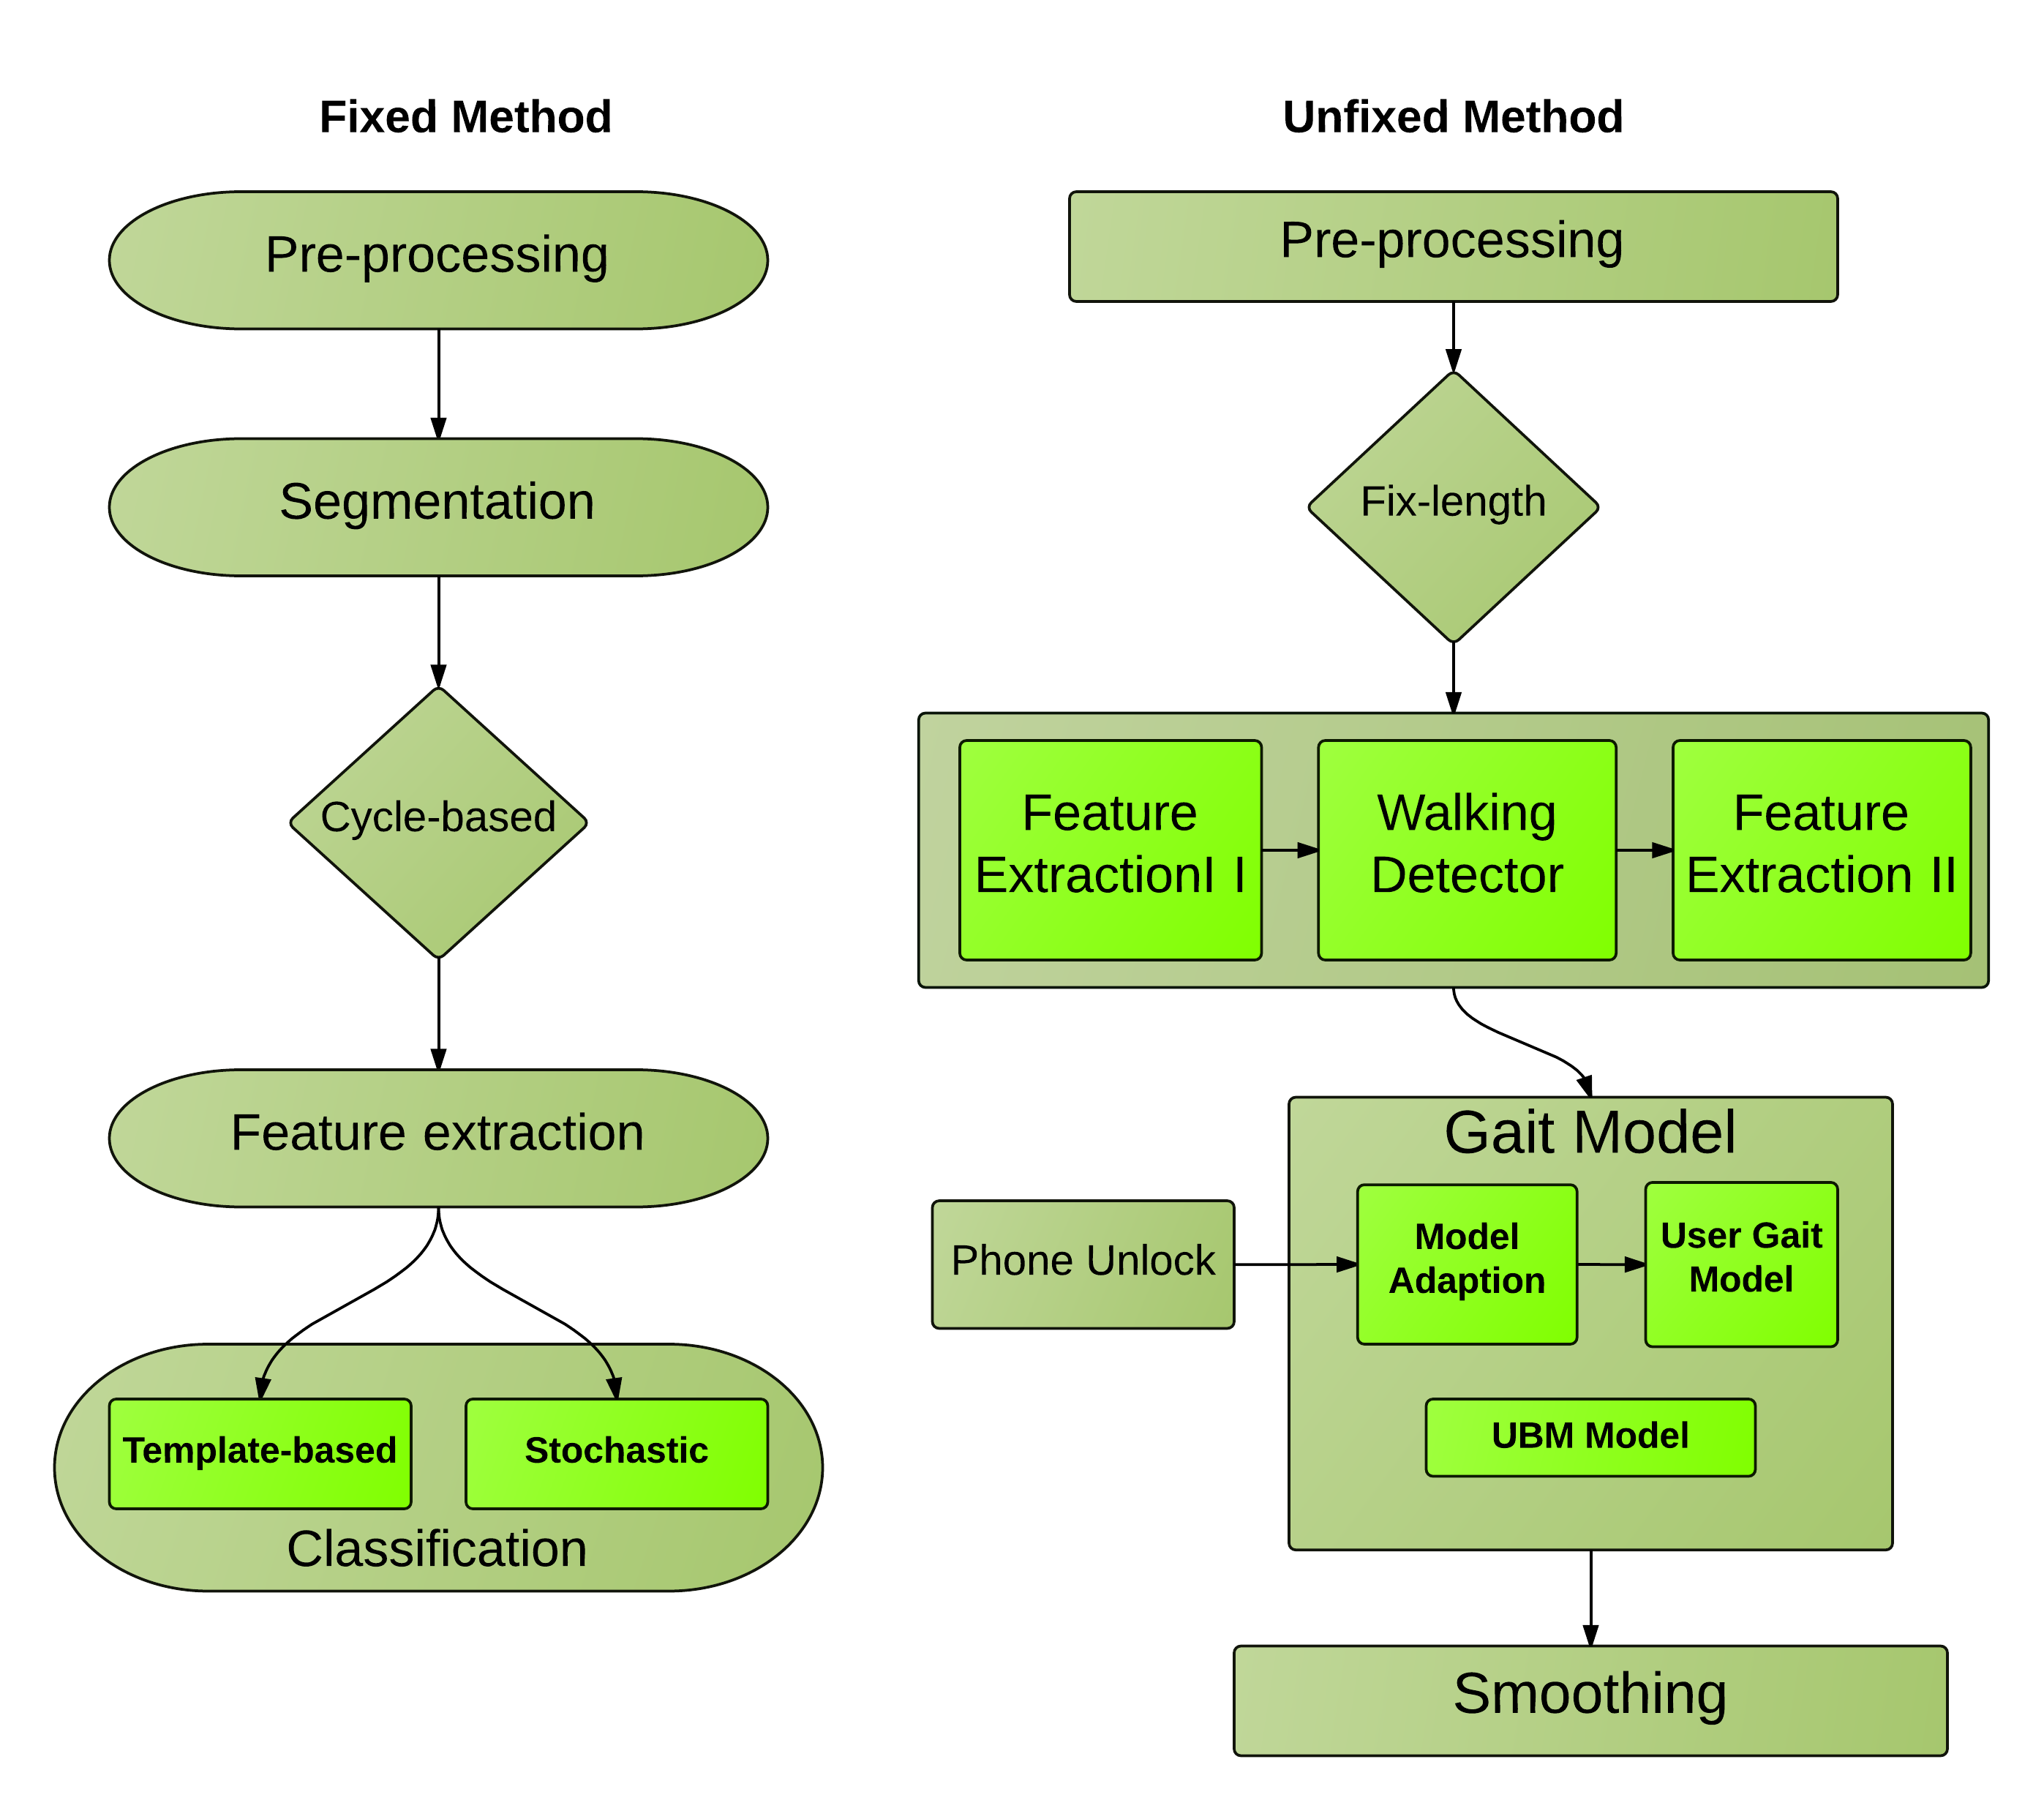
\psfig{file=AlgorithmProcess.png,height =3.2in, width =3.8in}
\caption{Different Approaches}
\label{fig:AlgorithmProcess}
\end{figure}	
%@@@@@@@@@@@@@@@@@@@@@@@@@@@@@@@@@@@@@@@@@@@@@@@@%%

%I plan to use the following sources:
%\begin{itemize}
%\item one~\cite{Sujithra:2012}
%\item two~\cite{Muaaz:2013}
%\item three~\cite{Lu:2014}
%\end{itemize}


%----------------------------------------------------------------------------------------------------------------------%
\section{Background}
	Biometrics can be used as a new form of security that provides unique identification to a mobile user. Instead of relying on a password or physical key, a person can gain access to their device by a physical characteristic specific to them. Biometrics can be split into two categories, physiological and behavioural. Physiological biometrics include: Finger Scan, Facial Scan, Iris Scan, and DNA Matching. Behavioural biometrics include: Voice Recognition, Keystroke Scan, and Gait Recognition. In this paper, I will focus on gait recognition. The term gait refers to the walking pattern of a person. A person's walking pattern is cyclic in nature and may be composed of many gait cycles, where each gait cycle consists of at least two steps.~\cite{Sujithra:2012} 
	
	In mobile security, when gait recognition is used, gait data is collected via the built-in accelerometer of the smart phone. The smart phone will use the collected data to analyze a person's walking pattern. If the phone can determine that the current user should have access, the phone will be unlocked. Otherwise the phone will switch to a different authentication method such as pin access. This method increases the security of the mobile device, because the form of unlocking the device is now a person characteristic (a biometric) and not something that is likely stolen or forgotten. Also, unlike other biometrics, such as a fingerprint that can be copied, an imposter would have trouble replicating a gait pattern.


%----------------------------------------------------------------------------------------------------------------------%
\section{Pre-processing} 
	Once data is gathered, it needs to be pre-processed into a usable form which is done by separating the data into pieces. In the following sections I will explain the fixed and unfixed methods of pre-processing.

    %\\\\\\\\\\\\\\\\\\\\\\\\\\\\\\\\\\\\\\\\\\\\\\\\\\\\\\\\\\\\\\\\\\\\\\\\\\\\\\\\\\\\\\\\\\\\\\\\\\\\\\\\%
\subsection{Fixed Method Pre-processing}	
	With the phone on the waist in a fixed position, uniform sets of data called \textit{walks} were collected. One walk is defined by walking a measured distance down a hallway. The experiment was conducted so that one set of data contained two ``walks''. In other words, one set of data was walking down a hallway, once down and once back. After extracted, the raw gait data is pre-processed using two steps: \textit{linear interpolation} and \textit{zero normalization}. 
			%+++++++++++++++++++++++++++++++++++++++++++++++++++++++++++++++++++++++++++++++++++%
\subsubsection{Linear Interpolation} 
	Since the built-in accelerometer does no output data in equal intervals, the data needs to be reshaped into equal intervals. This is done by applying \textit{linear interpolation}. To avoid losing data during this change, up-sampling can be applied. Up-sampling avoids data loss by producing ``an approximation of the sequence that would have been obtained by sampling the signal at a higher rate''~\cite{wiki1:2014}. Once the data has been reshaped, the acceleration measurements have to be adjusted to account for unstable accelerometer readings. 
			%+++++++++++++++++++++++++++++++++++++++++++++++++++++++++++++++++++++++++++++++++++%
\subsubsection{Zero Normalization}
	The mobile device's accelerometer is used to measures 3 axes (X, Y, Z). The only axis needed, and the only axes affected by gravity is the X axis. Since the acceleration for the Y and Z axis are not stable over time, and they are not affected by earth's gravity, the acceleration data for the Y and Z axis have to be \textit{zero normalized}. In other words the data for the Y and Z axes have to be set to zero. This is done by simply subtracting their total acceleration from their average acceleration. An overview of the stages explained above are shown in figure ~\ref{fig:firstStep}.
	
%@@@@@@@@@@@@@@@@@@@@@@@@@@@@@@@@@@@@@@@@@@@@@@@@%
\begin{figure}
\centering
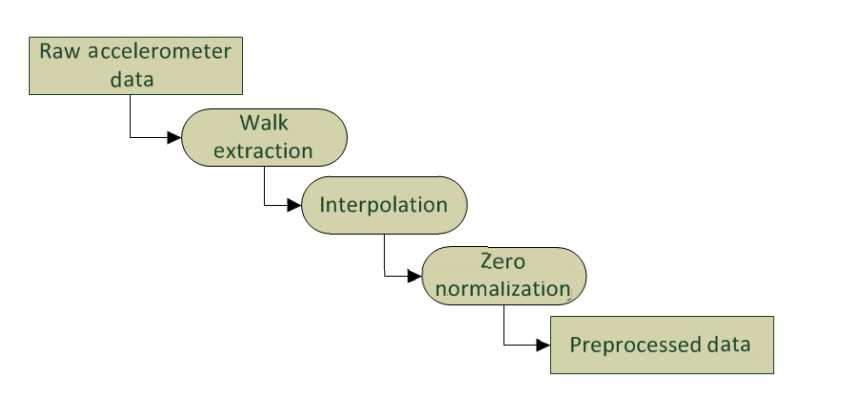
\psfig{file=chart1.png,width =3in}
\caption{Fixed Method Pre-processing Step}
\label{fig:firstStep}
\end{figure}

%@@@@@@@@@@@@@@@@@@@@@@@@@@@@@@@@@@@@@@@@@@@@@@@@%
	%\\\\\\\\\\\\\\\\\\\\\\\\\\\\\\\\\\\\\\\\\\\\\\\\\\\\\\\\\\\\\\\\\\\\\\\\\\\\\\\\\\\\\\\\\\\\\\\\\\\\\\\\%
\subsection{Un-fixed Method Pre-processing}{
	The previous method used a phone in a fixed location. This method expands from having the phone on the waist, to having the phone in a unfixed location, such as a pocket. Also, this method does not use a set length, such as a hallway, making it more flexible. To mark each walk this method uses a process called \textit{framing}. Framing separates the data into sets of equal time. Once the data is segmented into frames, it is then projected onto a global coordinate system through a process know as \textit{projection}.}
		
		
			%+++++++++++++++++++++++++++++++++++++++++++++++++++++++++++++++++++++++++++++++++++%
\subsubsection{Framing}{
 During Framing, sensor data is segmented into uniform frames for feature extraction and feature classification. This is similar to the pre-processing of the data for the fixed method. The fixed method had its data separated into ``walks''. This data, not having the separation of ``walks'', is separated into sections of 512 equal samples in length. This is done by separating sections every 5.12 seconds. They state the reason for 512 samples was ``to balance between estimation accuracy and latency.'' In other words, this was to balance between the accuracy of matching a user and the time it took to compute the match. Also, not all frames move onto feature extraction. Frames that are below a chosen threshold, representing no movement, are dropped. }
 			%+++++++++++++++++++++++++++++++++++++++++++++++++++++++++++++++++++++++++++++++++++%
\subsubsection{Projection}{
	Each sample within a given frame contains an X, Y, and Z coordinate. Each coordinate is then projected into a vertical and horizontal variable. Once each sample is projected, the direction of gravity is determined by using a mean filter. Unlike the previous example, this process does not assume a fixed location or orientation of the mobile device. In order for the device to record accurate data from the accelerometer, the devices orientation (up, down, left, and right) must be accurate. If there is a significant change in the gravity variable then the orientation of the device has changed. This means the corresponding frame will be dropped and the horizontal and vertical axes will be adjusted accordingly. 
}
\subsection{Comparison of Pre-processing Approaches}
	Both the fixed and unfixed method split the data into equal intervals as well as modify the data so that it is in a useful form. The reason for the differences between the pre-processing methods stems from the differences in phone placement. The data collected in the fixed method is already more organized than the data from the unfixed method. This is because the unfixed method has to account for multiple axes as well as data unrelated to gait. If the fixed method were to be implemented in more of a real life scenario then these methods become even more similar. 




%----------------------------------------------------------------------------------------------------------------------%
\section{Feature Extraction}
	\textit{Feature Extraction} is extracting a set of data from a given frame to detect patterns of walking. Another way to define feature extraction is the process of extracting gait cycles from the data. 		%\\\\\\\\\\\\\\\\\\\\\\\\\\\\\\\\\\\\\\\\\\\\\\\\\\\\\\\\\\\\\\\\\\\\\\\\\\\\\\\\\\\\\\\\\\\\\\\\\\\\\\\\%
\subsection{Fixed Method Feature Extraction}
	The fixed method uses the following steps in order, as seen in Figure~\ref{fig:SecondStep}: Cycle length estimation, Cycle detection, Cycle length normalization, Omitting unusual cycles. 
	
%@@@@@@@@@@@@@@@@@@@@@@@@@@@@@@@@@@@@@@@@@@@@@@@@%
\begin{figure}
\centering
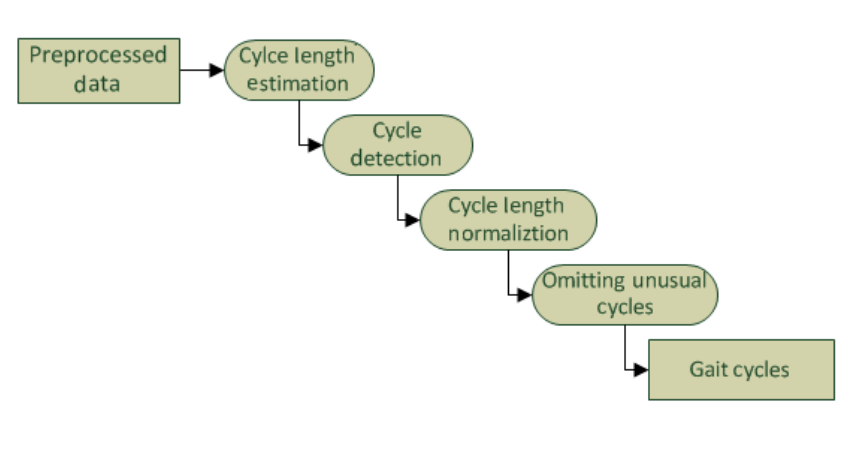
\psfig{file=chart2.png,width =3in}
\caption{Feature Extraction}
\label{fig:SecondStep}
\end{figure}

%@@@@@@@@@@@@@@@@@@@@@@@@@@@@@@@@@@@@@@@@@@@@@@@@%
			%+++++++++++++++++++++++++++++++++++++++++++++++++++++++++++++++++++++++++++++++++++%
\subsubsection{Cycle Length Estimation}
Once the raw gait data is pre-processed, the next step is extracting the biometric gait cycles. The first step in extraction is to be able to automatically detect gait cycles in the walk. This detection is done by estimating the cycle length, which is simply computing \textit{minimum salience vector}. For this instance a salience vector is distance measurement from one point of a cycle to another. There is a minimum salience vector for each data point for a given walk. Each minimum salience vector is computed by counting the data values that are between the current data value and the following smaller value in the walk vector. The number of values counted is the current points distance measurement. The salience vector with the greatest distance measurement is considered a cycle start. 
			%+++++++++++++++++++++++++++++++++++++++++++++++++++++++++++++++++++++++++++++++++++%
\subsubsection{Cycle Detection}
Once both minimum and maximum salience vectors are computed, they can be used to detect individual cycles. Figure~\ref{fig:AccelChart} shows a set of gait cycles in black, and the salience vector distance measurement in grey. The start of each cycle is based on the minimum salience vector. Around times 750, 1150, 1450, and 1650 can be seen spikes where the distance measurement is larger than the rest. These spikes are the minimum salience vectors, marking the start of gait cycles. This same process is applied to determine the maximum salience vector as well. If there are some cycle that are much longer than others, these minimum and maximum points are used to determine more cycle starts. This splits too long cycles into smaller ones.

%@@@@@@@@@@@@@@@@@@@@@@@@@@@@@@@@@@@@@@@@@@@@@@@@%
\begin{figure*}
\centering
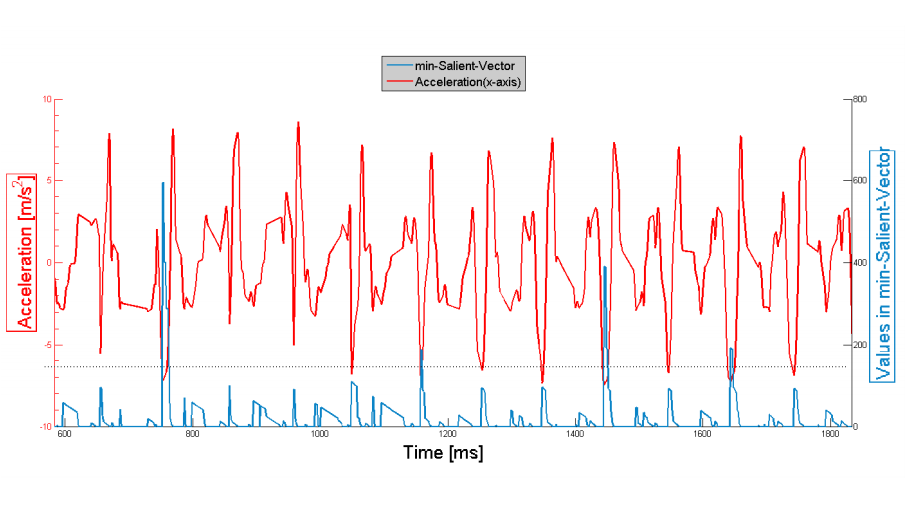
\psfig{file=svector.png,height =2.5in,width =5.3in}
\caption{Minimum Salient Vectors}
\label{fig:AccelChart}
\end{figure*}

%@@@@@@@@@@@@@@@@@@@@@@@@@@@@@@@@@@@@@@@@@@@@@@@@%
			%+++++++++++++++++++++++++++++++++++++++++++++++++++++++++++++++++++++++++++++++++++%
\subsubsection{Cycle Length Normalization}
Once each start of a cycle is determined, the cycle distance is the distance from the start of one cycle to the start of the following cycle. Each cycle does not have the same length. By using linear interpolation, the determined cycles are normalized to a set length. Equal cycle lengths are later required for some feature extraction techniques. 
			%+++++++++++++++++++++++++++++++++++++++++++++++++++++++++++++++++++++++++++++++++++%
\subsubsection{Omitting Unusual Cycles}
Some cycles compared to the majority are considered unusual. These could be caused by any motion or non-motion that does not correspond to walking. Such patterns are detected by ``computing the distance using \textit{Dynamic Time Warping} (DTW).''~\cite{Muaaz:2013} Dynamic time warping is ``an algorithm for measuring similarity between two temporal sequences which may vary in time or speed.''~\cite{wiki2:2014} This means that cycles with an acceleration of half or more of the other cycles will be removed



    %\\\\\\\\\\\\\\\\\\\\\\\\\\\\\\\\\\\\\\\\\\\\\\\\\\\\\\\\\\\\\\\\\\\\\\\\\\\\\\\\\\\\\\\\\\\\\\\\\\\\\\\\%
\subsection{Unfixed Method Feature Extraction}
	A different form of extraction used by~\cite{Lu:2014} is a combination of time-domain, frequency-domain, and auto-correlation features. This example also did feature extraction in two stages: calculating the set of features for walking and calculating more precise gait features. 
%@@@@@@@@@@@@@@@@@@@@@@@@@@@@@@@@@@@@@@@@@@@@@@@@%
\begin{figure}
\centering
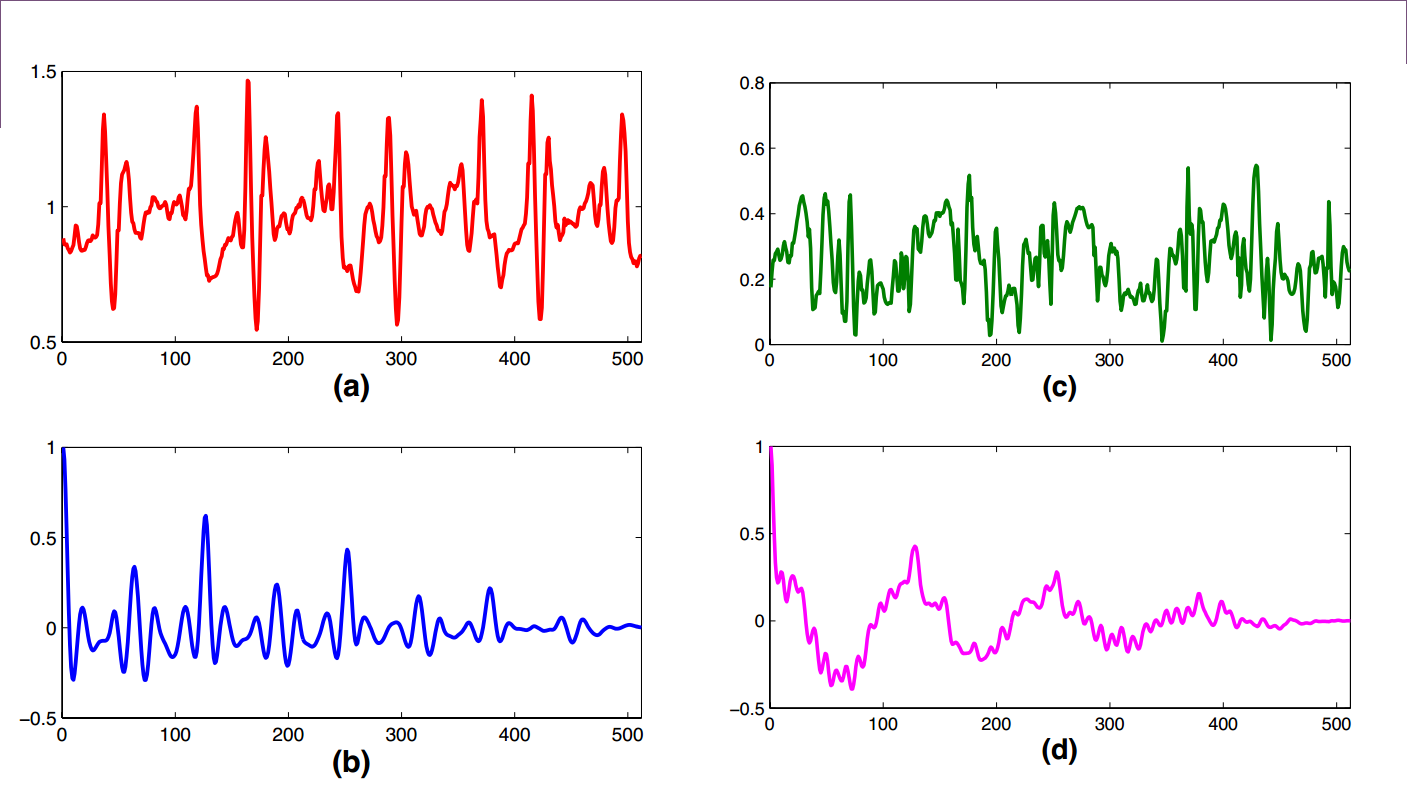
\psfig{file=abcd.png,width =3in}
\caption{(a) projected vertical component. (b) normalized autocorrelation of the vertical component. (c) projected horizontal component. (d) normalized autocorrelation of the horizontal component}
\label{fig:TD1}
\end{figure}

%@@@@@@@@@@@@@@@@@@@@@@@@@@@@@@@@@@@@@@@@@@@@@@@@%	%+++++++++++++++++++++++++++++++++++++++++++++++++++++++++++++++++++++++++++++++++++%
\subsubsection{Feature Extraction I}
	The first stage of the feature extraction is used to tell whether or not the data represents walking data. This is done to rule out the times when the mobile device is not collecting the right data. For example if the mobile device was collecting data when it was in a car going down the road, that data should not be used because it is not gait data. This also holds true for collecting data on someone who is standing still. The data collected would not represent the data needed for a biometric. Telling whether the data collected is of someone walking is done by collecting vertical and horizontal features to produce motion patters. Six time-domain features are used for both directions. These six feature are :mean, variance, skewness, kurtosis, energy, mean-crossing rate. All these features are based on spectrum analysis. In other words, doing ``different activities have different energy distributions over the frequency spectrum.''~\cite{Lu:2014} Walking can be measured around 1-2Hz while driving in a car will output a higher frequency band. Based on these frequency levels the data is put into one of three classes: walking, non-walking and motion(high frequency movement such as a in a vehicle or running).~\cite{Muaaz:2013}
			%+++++++++++++++++++++++++++++++++++++++++++++++++++++++++++++++++++++++++++++++++++%
\subsubsection{Walking Detection}
	Using data from Feature Extraction I, classification can be done using a decision tree.There are three activities that the data can be classified as: walking, non-walking, and random movements. Non-walking motion is running, biking, or moving in a vehicle. Random motion is a motion such as turning or skipping. A Markov Model smoother is applied to the new set of data to get rid of any outliers. 
			%+++++++++++++++++++++++++++++++++++++++++++++++++++++++++++++++++++++++++++++++++++%
\subsubsection{Feature Extraction II}{
	Feature extraction II is done once the data collected is determined to be gait data. In this stage more relevant features are extracted for analysis. The first analysis to be done is the Compressed sub-band cepstral coefficients(CSCC). This is done in the following three steps. First, the energy spectrum is computed using the FFT spectrum. The Fast Fourier Transform(FFT) is an alogorithm that computes the Discrete Fourieer Transform(DFT) and its inverse. The study maps the energy spectrum into 26 bands using triangular overlapping bands and sum up the energy in each band. The processing then takes the discrete cosine transform of the sub-band energy to form a 12-dimension vector representation. This in all summarizes the fundamental frequency of the movements and the higher frequency vibrations in the data.~\cite{Sujithra:2012}
}
	Both of these methods of feature extraction try to determine what parts of the data represent a walk cycle. The fixed method is simpler because it does not have to worry about different variables affecting the data. Though this method is simpler, it has the stipulation of the mobile device being clipped to your waste. The non-fixed method has to worry about more variables affecting the data, but implements a real life situation of just having the mobile device in a pocket.
	
	
	
		
%----------------------------------------------------------------------------------------------------------------------%
\section{Gait Classification}
	This last step is taking the extracted features and verifying that those features match a stored set of features; the stored set of features being the users. The fixed method uses Support Vector Machines(SVM's). The basic idea of SVM's is taking dimensional data and separating it into two classes. This involves the use of a Gaussian kernel defined in the following section. The unfixed method uses a Gaussian Mixture Model - Universal Background Model(GMM-UBM) framework to verify a individuals gait. The basic idea with this technique is with scoring. Verification of a users identity is done by comparing the likelihood score from a users gait pattern to the universal back ground model. The universal back ground model represents human gait patterns in general
   %\\\\\\\\\\\\\\\\\\\\\\\\\\\\\\\\\\\\\\\\\\\\\\\\\\\\\\\\\\\\\\\\\\\\\\\\\\\\\\\\\\\\\\\\\\\\\\\\\\\\\\\\%
\subsection{Fixed Method Gait Classification}\label{FMGC}
	SVMs are another way to classify gait data. SVMs are often used for biometric recognition, where imposter and genuine data have to be determined. First the SVM finds a \textit{hyperplane}. A hyperplane is a subspace that is one dimension less than its ``ambient space''. For example, there could be a set of data represented by 3 axis (X,Y,Z). The hyperplane would be the same data plotted on a 2 axis space. So, the SVM will take the data, and find a hyperplane that linearly separates \begin{math}\mathcal{D} \end{math} dimensional data into two classes. The dimensional data has to be linearly separable for the SVM to work. Since the gait data is not linearly separable, a ``kernel induced feature space''~\cite{Muaaz:2013} is introduced in the SVM. A kernel function maps non linearly separable data to a high dimensional space. Once mapped to a high dimensional space the data is linearly separable and therefore can be used by the SVM to find a hyperplane. This means that depending on the kernel function you use, the better classification accuracy it will produce. 
% Reword this to get rid of euclidean distance.	
%	Another more commonly used kernel function is the Gaussian kernel, which uses the Euclidean distance. Since the Euclidean distance restricts to only using fixed length cycles, 
There are kernel functions that would require the use of fixed length gait cycles. Since gait cycles are not usually of a fixed length, a different kernel is used. By using the DTW distance, the problem of fix-length input feature vectors can be solved as well as more accurate finding of similarity in the data. Two different approaches using SVM and DTW can be used to classify gait cycles:Pre-computed data matrix, and Pre-computed kernel. ~\ref{fig:TrainingData}
	

%@@@@@@@@@@@@@@@@@@@@@@@@@@@@@@@@@@@@@@@@@@@@@@@@%
\begin{figure}
\centering
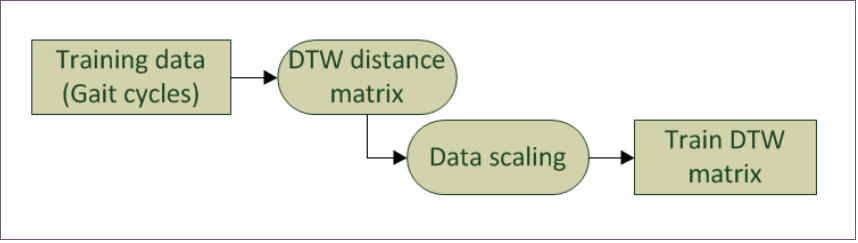
\psfig{file=TrainingData.png,width =3in}
\caption{Preparing data for SVM)}
\label{fig:TrainingData}
\end{figure}

%@@@@@@@@@@@@@@@@@@@@@@@@@@@@@@@@@@@@@@@@@@@@@@@@%	
	
%+++++++++++++++++++++++++++++++++++++++++++++++++++++++++++++++++++++++++++++++++++%
\subsubsection{Pre-computed data matrix}
	Gait cycles are represented by the DTW distance. The DTW distance is the distance between two gait cycles. The benefit of the DTW distance is that gait cycles with different length can be found. A DTW matrix is then computed by taking the sample DTW distance and compared to all other samples. This matrix is needed as an input for the SVM.	
			%+++++++++++++++++++++++++++++++++++++++++++++++++++++++++++++++++++++++++++++++++++%
\subsubsection{Pre-computed Kernel}
Using GDTW kernel equation ~\ref{eq:KF3} as the kernel matrix also allows to classify the gait data. Though this kernel matrix is a symmetric matrix, it is not guaranteed that it has all positive eigenvalues. 
\begin{equation} \label{eq:KF3}
K(x,z)=exp(-\gamma \parallel DTW(x,z) \parallel ^2)
\end{equation}	
    %\\\\\\\\\\\\\\\\\\\\\\\\\\\\\\\\\\\\\\\\\\\\\\\\\\\\\\\\\\\\\\\\\\\\\\\\\\\\\\\\\\\\\\\\\\\\\\\\\\\\\\\\%
\subsection{Unfixed Method Gait Classification}
The framework used for classifying gait cycles is a Gaussian Mixture Model-Universal Background Model (GMM-UBM). The algorithm can be split into three primary sections: UBM training, user gait model genertion, runtime inference and adaptation. 

	 The UBM is a large Universal background GMM that is trained from a large source of data. This means a UBM represents the general walk pattern of humans. The UBM is defined as 
\begin{math} \lambda \end{math} (\begin{math} \omega \end{math},
\begin{math} \upmu \end{math},
\begin{math} \Sigma \end{math}) where
\begin{math} \omega \end{math} represents the mixture weight, \begin{math} \upmu \end{math} represents the mean, and \begin{math} \Sigma \end{math} represents the covariance matrix. In other words \begin{math} \omega \end{math} is the prior distribution of waling patterns while \begin{math} \upmu \end{math} and \begin{math} \Sigma \end{math} are different walking patterns given by the population in different conditions. For efficiency the \textit{covariance matrix} is used. A covariance matrix ``generalizes the notion of variance to multiple dimensions.'' Also, to avoid over fitting the training data, a standard expectation maximization (EM) algorithm is applied. The EM is what trains the UBM models. For example, if given a collection of training vectors, the EM estimates the parameters to most likely to occur. The EM algorithm does this through iteration. Each time the algorithm iterates it refines the GMM parameters, increasing the likelihood of the estimated model for the given feature vectors. 
%maybe provide an example?????
	The individual user's gait model is a GMM, but instead of using EM training, a Bayesian adaptation is used. This is simply relating the odds of one event to the odds of another. The use of the Bayesian adaptation is both used for performance as well as for its ability to learn from the data. The Maximum-a-Posteriori (MAP) is the adaptation used. The MAP adaptation adjusts the Gaussian components and mixture weight to personalize the UBM model. 
	It is during runtime when the extracted features are compared against the user gait model and the UBM creating a score. High scores result from the user model being higher than the UBM model and visa versa for low scores. The score are computed as \begin{equation}
	\Updelta = log(p(X|\lambda_{user})) - log(p(X|\lambda_{ubm}))
	\end{equation}
In this equation \begin{math} \Updelta \end{math} is equal to the users score, X is the feature vector, and \begin{math} \lambda \end{math} represents the type of model the feature vector is being compared against. MAP is also ran at runtime to learn new gait patterns from the user. It does the from false negatives given to the device by an alternative form of authentication. 

%@@@@@@@@@@@@@@@@@@@@@@@@@@@@@@@@@@@@@@@@@@@@@@@@%
\begin{figure}
\centering
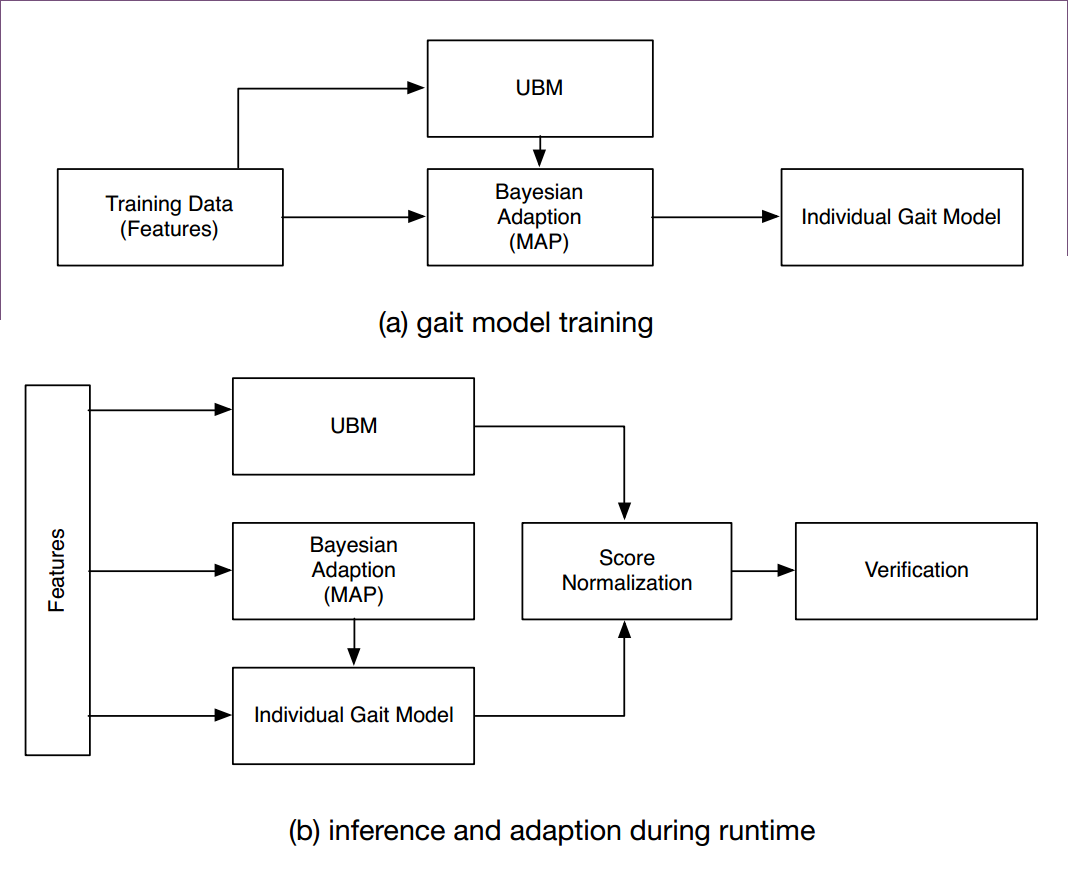
\psfig{file=FESP.png,width =3in}
\caption{Algorithm work-flow for (a) generate user gait model by MAP adaptation (b) runtime inference and Individual model adaptation}
\label{fig:TD2}
\end{figure}
%@@@@@@@@@@@@@@@@@@@@@@@@@@@@@@@@@@@@@@@@@@@@@@@@%
%----------------------------------------------------------------------------------------------------------------------%
%\section{Experiment Results}
%\subsubsection{Paper 1(title place holder)}
%\subsubsection{Paper 2(title place holder)}


%----------------------------------------------------------------------------------------------------------------------%
\section{Putting it all Together}
I have compared two forms of using built gait as a form of mobile security. One experiment used a fixed location for the device while the other used multiple locations. Both use different methods of extracting the gait data as well as well as analyzing the data, but each method does use a popular Android phone. Both of these experiments are not perfect yet but they both show promise in using walking patterns as a form of mobile security.
	%\\\\\\\\\\\\\\\\\\\\\\\\\\\\\\\\\\\\\\\\\\\\\\\\\\\\\\\\\\\\\\\\\\\\\\\\\\\\\\\\\\\\\\\\\\\\\\\\\\\\\\\\%
\subsection{Fixed Method Experiment}
	The Fixed method did two experiment setups: Template-based classification and Machine learning based classification. The data set was made from 51 subjects (39 males, 12 females) that walked down a 18.5 meter long corridor.
			%+++++++++++++++++++++++++++++++++++++++++++++++++++++++++++++++++++++++++++++++++++%

%@@@@@@@@@@@@@@@@@@@@@@@@@@@@@@@@@@@@@@@@@@@@@@@@%
\begin{figure}
\centering
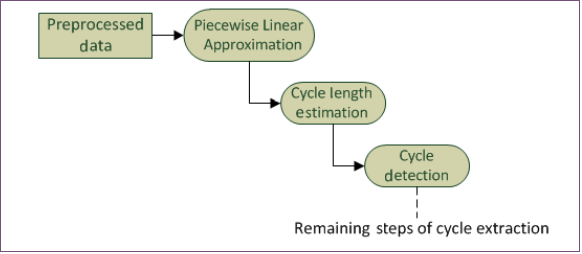
\psfig{file=PreprocessedData.png,width =3in}
\caption{Gait cycle extraction steps with Piecewise Linear Approximation(PLA)}
\label{fig:AddedStep}
\end{figure}
%@@@@@@@@@@@@@@@@@@@@@@@@@@@@@@@@@@@@@@@@@@@@@@@@%
\subsubsection{Template-based classification}
	 For the template-based classification a interpolation of 100 Hz was used. Also, for this experiment a Piecewise Linear Approximation (PLA) was used before the cycle length estimation step. A PLA is a function that is used to approximate a curve connecting points along the curve with straight lines (interpolating linearly). Also, the PLA uses the Sliding Window And Bottom-up (SWAB) approach. The SWAB approach starts at the leftmost detected segment, applies the PLA function, and moves onto the new set of data using the sliding window approach. It is this PLA representation of the walks that will undergo the remaining steps. From the final processed data, the best cycle with the lowest DTW distance is chosen. This cycle is known as the feature cycle. the remaining cycles are known as probe cycles. Once all the reference and probe cycles are computed two classes are made: genuine and impostor. These classes are made by comparing the two classes against one another in respect to their DTW distances. If at least 50\% of one walk votes for the genuine class then accept, else reject. The accuracy of this method is measured by the Equal Error Rate (EER). This is the rate ate which both the acceptance and rejection errors are equal. For this template-based classification the EER was 22.49\% for same-day, 29.4\% for different-day and 33.3\% for mixed days. 
	 			%+++++++++++++++++++++++++++++++++++++++++++++++++++++++++++++++++++++++++++++++++++%
\subsubsection{Machine learning based classification}
The machine learning classification uses the normal approach to processing the data along with the added approaches described in section \ref{FMGC}. Once the gait cycles are extracted they are separated, 80\% go into a training data set while 20\% go into a testing data set. The DTW distance matrix is computed using the training data set. 
\subsection{UnFixed Method Experiment}
	The Unfixed method experimented using 3 data sets all using android phones. The first data set included 49 people, 19 female and 28 male. These subjects performed various tasks that included: standing, sitting, walking, biking, running, driving, and random movements. The second data set was made up of 12 people, 5 female and 7 male. These subjects did tests in a more controlled environment with different phone placements, walking distances, and walking speeds. The third data set was to collect data in a real-world setting. This involved 8 people that collected data for 5 hours each.

\section{Conclusion}
	I have compared two forms of gait recognition methods using very similar strategies to create an unobtrusive security process for mobile phones using stock android phones. The difference between these two methods are: placement of the mobile device, and their different implementations of of the strategies to which their algorithms were built. Though the fixed method was more geared to a controlled setting and the unfixed method was geared to more real world implementations, they both show promise for future work. 
	
	The fixed method used a new method to extract gait cycles using Piecewise Linear Approximation. The fixed method also used two new approaches using Support Vector Machines and Dynamic Time Warping to classify gait cycles. Though only gait cycles of the same length were used, DTW allows for future work with gait cycles of variable lengths. Future work will involve recording at higher sampling rate (varying frequencies) as well as placing the phone in more realistic positions on the body.
		
		The unfixed method used a different approach when dealing with gait data. There was the use of MAP and Gaussian Mixture Models, customizing the gait model. Future work will involve training the UBM better by sampling from a larger data set. There are also trade-offs to be made balancing performance over usability. Using a longer smoothing window could help improve accuracy but will take longer to verify the user.
%----------------------------------------------------------------------------------------------------------------------%
\section{Acknowledgments}
	I would like to thank Kristin Lamberty, and Elena Machkasova for their advice and feedback as well as Melissa Helgeson for additional feedback and proofreading. 
% The following two commands are all you need to
% produce the bibliography for the citations in your paper.
\bibliographystyle{abbrv}
% annotated_bibliography.bib is the name of the BibTex file containing 
% all the bibliography entries for this example. Note that you *don't* include the .bib ending
% in the \bibliography command.


%----------------------------------------------------------------------------------------------------------------------%
\bibliography{paper}  

% You must have a ".bib" file and remember to run:
%     pdflatex bibtex pdflatex pdflatex
% in order to see all the citation references correctly.







%
%\begin{displaymath}
%K : X \times X \rightarrow \mathbb{R}, \forall \{x,z\} \in X
%\label{eq:KF1} 
%\end{displaymath}
%
%\begin{displaymath}
%K(x,z)=< \phi (x).\phi(z) > 
%\label{eq:KF2}
%\end{displaymath}

\end{document}



